\section{Problemática}
En el proceso actual de la División de Innovación Academica de la Dirección de Educación Superior(DES), se identifico como área de oportunidad la elaboración y revisión de Programas de Estudio de las Unidades de Aprendizaje para la creación o rediseño de un Plan de Estudios. Debido a las siguientes situaciones:\\
\begin{itemize}
    \item Las unidades académicas no respetan el proceso estipulado para la creación de planes de estudio o unidades de aprendizaje.
    \item Los docentes no cuentan con una herramienta que los limite a los lineamientos en la elaboración del programa de estudios.
    \item El control de cambios para las unidades de aprendizaje se realiza de forma manual.
    \item No se cuenta con un control par administrar, organizar y/o distribuir unidades de aprendizaje que se realizan de manera manual.
    \item No existe una herramienta para gestionar los cambios o control de cambios solicitados por la DES a cada unidad de aprendizaje.
    \item Se exceden los tiempos establecidos para el diseño o rediseño de Programas Académicos.
\end{itemize}
\begin{figure}[H]
	\centering
	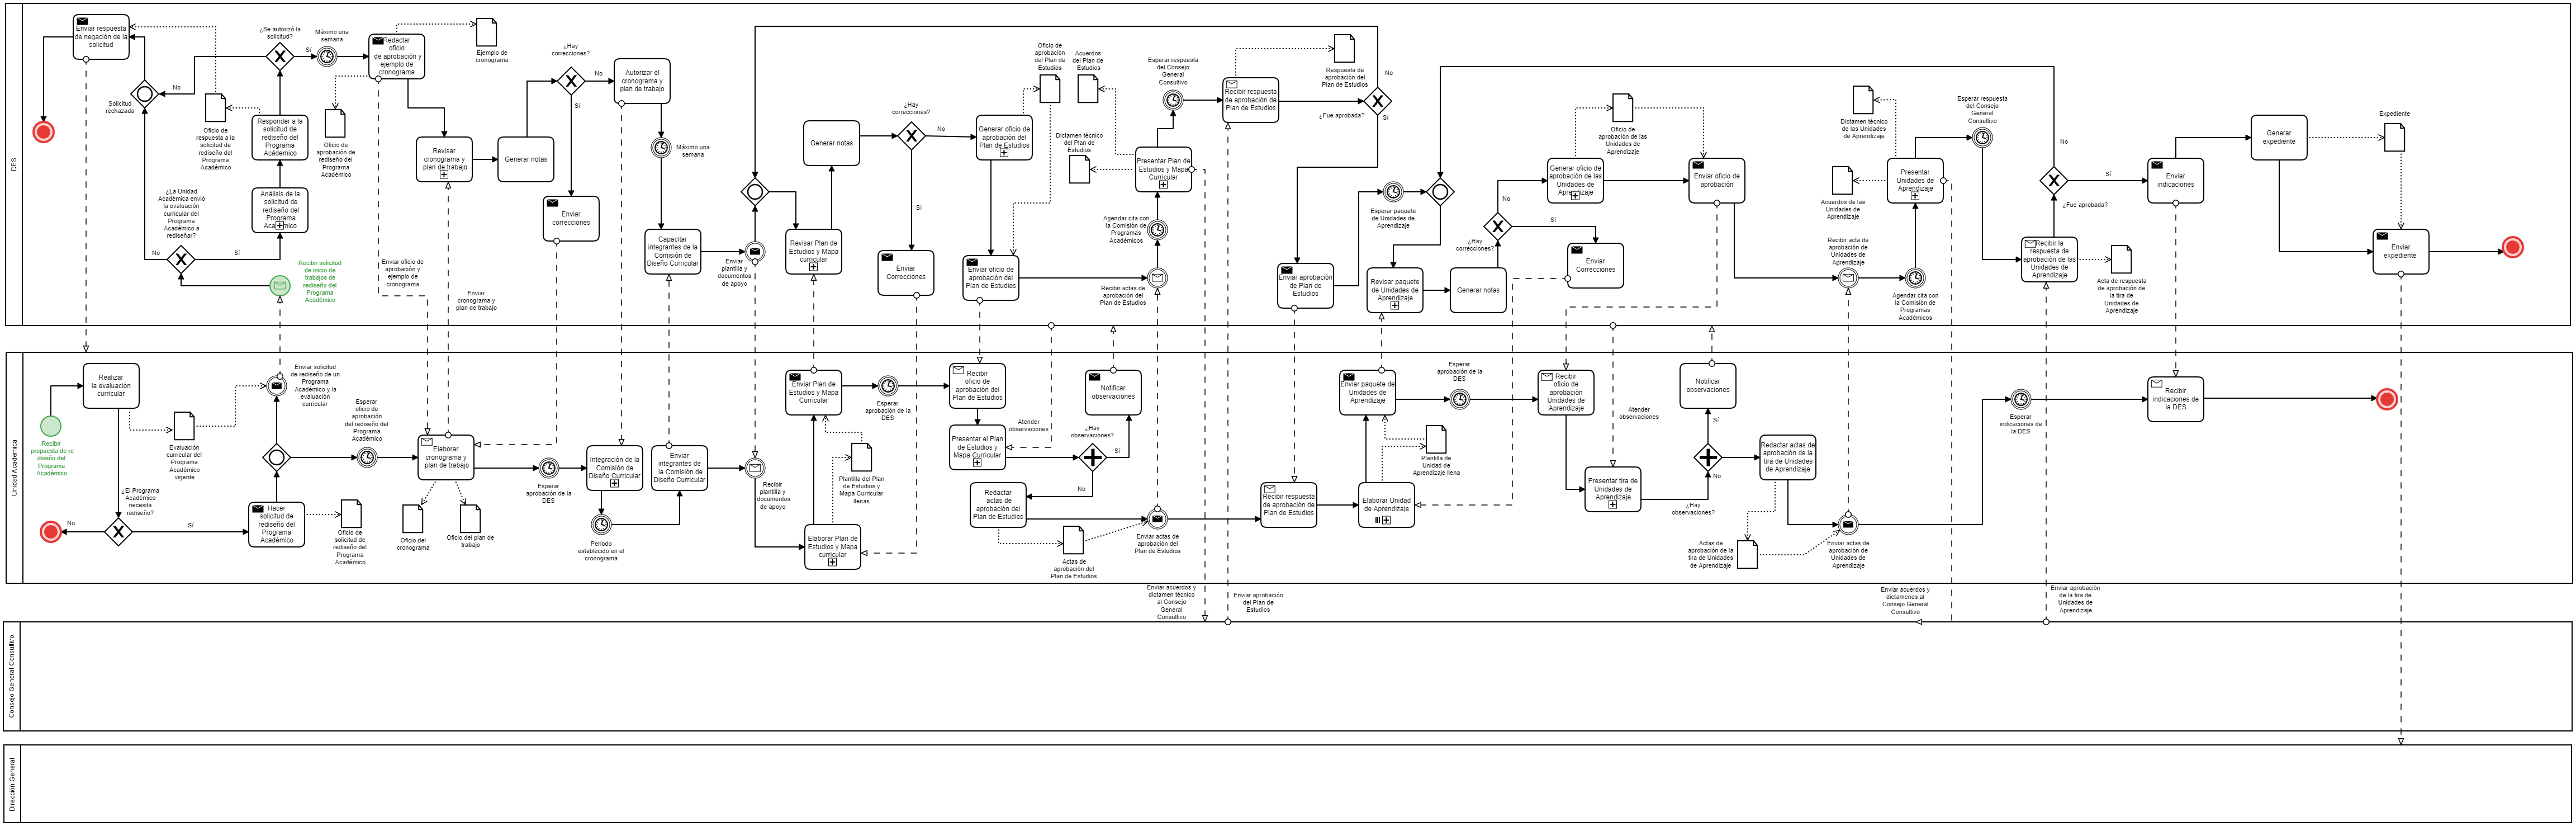
\includegraphics[width=0.9\linewidth]{images/Procesos/MacroProceso}
	\caption{Modelado del Negocio}
\end{figure}
